\documentclass[preprint,5p]{elsarticle}
\usepackage{graphicx}
\usepackage{dcolumn}
\usepackage{bm}  
\usepackage{amssymb}  
\usepackage{hyperref}
\providecommand{\keywords}[1]{\textbf{\textit{Index terms---}} #1}
\hypersetup{colorlinks=true, urlcolor=blue, citecolor=blue}
\usepackage[displaymath]{lineno}

%\linenumbers
%\linespread{2.5}

\title{\vspace{-15mm}\fontsize{18pt}{10pt}\selectfont\textbf{Rate capability 
and magnetic field tolerance measurements of fast timing microchannel plate 
photodetectors}}
\input author_list.tex  
\date{\today}
\begin{document}


\begin{abstract}
Microchannel plate photodetectors provide both picosecond time resolution and 
sub-millimeter position resolution, making them attractive photosensors for 
particle identification detectors of a future U.S. Electron Ion Collider. We 
have tested the rate capability and magnetic field tolerance of 6$\times$6 
cm$^{2}$ microchannel plate photodetectors fabricated at Argonne National 
Laboratory. The microchannel plate photodetector is designed as a low-cost 
all-glass vacuum package with a chevron pair stack of next-generation 
microchannel plates functionalized by atomic layer deposition. The rate 
capability test was performed using Fermilab's 120 GeV primary proton beam, and 
the magnetic field tolerance test was performed using a solenoid magnetic with 
tunable magnetic field strength up to 4 Tesla. The measured gain of the 
microchannel plate photodetector is stable up to 75 kHz/cm$^{2}$, and varies 
depending on the applied magnetic field strength and the rotation angle 
relative to the magnetic field direction.
\end{abstract}

\maketitle

\begin{keywords}
   Fast timing, Microchannel plate, Photodetector, Electron Ion Collider, 
   Particle identification detector, Rate capability, Magnetic field, Rotation 
   angle.
\end{keywords}


\section{Introduction} \label{sec:level1}
The world's first Electron Ion Collider (EIC) \cite{EIC} has been recommended
in the 2015 Long Range Plan for Nuclear Science as the highest priority for a 
new facility construction in the U.S following the completion of the Facility 
for Rare Isotope Beams (FRIB) \cite{LRP}. This unique facility will explore 
several features of the strong force and QCD through mapping the partons, 
quarks and gluons, content of nucleons and nuclei up to uranium, that will be 
accessible through processes such as semi-inclusive deep inelastic scattering 
and exclusive deeply virtual Compton scattering.  

Several detector concepts have been proposed and designed for the EIC at 
Argonne National Laboratory (ANL), Brookhaven National Laboratory (BNL), Thomas 
Jefferson National Accelerator Facility (JLab). For all these EIC detector 
designs, excellent particle identification (PID) ($e$/$\pi$/$K$/$p$) over a 
wide range of momentum is essential for the proposed measurements.  
Time-of-flight systems and imaging \u Cerenkov detectors, such as Ring Imaging 
\u Cerenkov (RICH)\cite{RICH,RICH2} and Detection of Internally Reflected \u 
Cerenkov light (DIRC) \cite{DRIC} detectors, are proposed. Both of these 
detector classes are calling for large area, low cost photon sensors with high 
spatial resolution, high rate capability, radiation tolerance, magnetic field 
tolerance, and picosecond timing resolution. 

Microchannel plate (MCP) photodetectors are compact photon sensors, usually 
with an internal chevron pair stack of MCPs. This  geometry provides both high 
spatial and temporal resolution in a vacuum package. The Large Area Picosecond 
Photodetector (LAPPD$^{TM}$) is the world's largest MCP based photodetector 
with an active area of 20$\times$20~cm$^2$ \cite{LAPPD}. It is designed as a 
modular all-glass detector package with the next-generation MCPs produced by 
applying resistive and emissive coatings to borosilicate glass capillary array 
(GCA) substrates through atomic layer deposition (ALD). The all-glass design 
and low-cost next-generation MCPs provide great advantages in reducing the 
LAPPD$^{TM}$ product cost per area compared to other currently available MCP 
based photodetectors. As a collaborating group of the LAPPD project 
\cite{LAPPD2}, we have built an MCP photodetector fabrication system 
\cite{LAPPD-ANL} at ANL to fabricate 6$\times$6~cm$^2$ MCP photodetectors with 
LAPPD design. The ANL's MCP photodetector fabrication system also serves as a 
an R{\&}D platform for LAPPD package design validation and optimization. 
Several 6$\times$6~cm$^2$ MCP photodetectors with standard LAPPD design were 
successfully fabricated at ANL and tested \cite{ANL-MCPs}-\cite{Wang-MCPs2}, 
exhibiting a high gain over 10$^7$, an overall time resolution of 35 ps, and a 
position resolution better than 1~mm. The excellent performance of these 
6$\times$6~cm$^2$ MCP photodetectors shows that the low-cost LAPPD$^{TM}$ 
detector is a promising candidate photosensors for the EIC PID detector 
systems. Performance tests of the MCP photodetectors in high rate, high 
radiation damage, and high magnetic field environments are required to further 
validate the application of LAPPD$^{TM}$ detectors as the EIC PID photosensors. 

In this paper, we describe the current design of 6$\times$6~cm$^2$ MCP 
photodetectors fabricated at ANL, report recent results on the performance 
tests of these 6$\times$6~cm$^2$ MCP photodetectors in a high rate environment 
and a high magnetic field environment. The direction of further optimization of 
the LAPPD$^{TM}$ design for an EIC PID application is also addressed at the end 
of this paper.


\section{Design of the MCP-based photodetector assembly} \label{sec_design}
The current ANL design of the 6$\times$6~cm$^2$ MCP photodetector is developed 
from the original LAPPD internal resistor chain design \cite{Wang-MCPs2}, 
similar to the current commercial standard design of LAPPD$^{TM}$ detectors 
\cite{Craven-MCPs}. Figure \ref{fig:design} shows a schematic design of the 
current ANL MCP-based photodetector assembly and its electrical circuit 
diagram.  

\begin{figure}[tbp]
\centering 
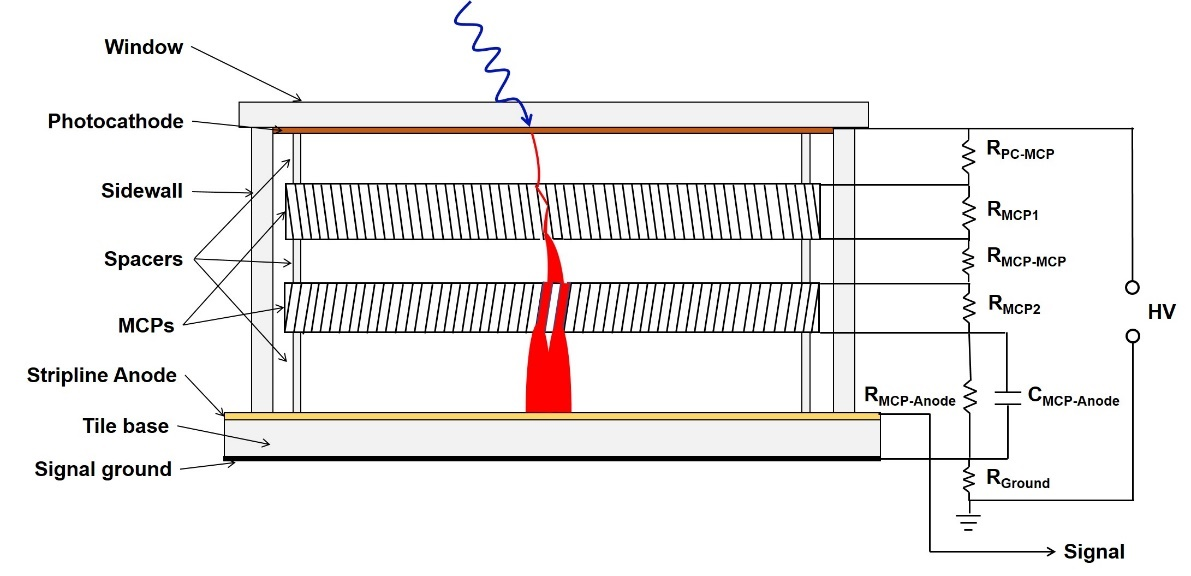
\includegraphics[scale=0.21]{fig/MCPs_design.png}
\caption{Schematic of MCP-based photodetector assembly (not to scale) and the 
   electrical circuit diagram. External connections to the top and bottom 
surfaces of the two MCPs are through ultra-thin metal shims (not shown) to 
special extra strip lines on the tile base. The circuit diagram shows 
connections through side wall in a simplified format.} 
\label{fig:design}
\end{figure}

The MCP photodetector is an all glass body assembly, consisting of a glass base 
window, a top window, two side walls, three grid spacers and two MCPs. The side 
walls are frit-bonded onto the base window, with silver stripline anodes 
printed to lead the signals and high voltage connections to the outside. Three 
grid spacer sets are used, one between the anode and the lower MCP, one between 
the two MCPs, and between the upper MCP and the top window. These spacers 
function as insulators to separate the different components, and also to hold 
these internal components in place in the vacuum assembly. 

Four ultra-thin metal shims are applied at the top and bottom surfaces of the 
two MCPs to lead the electrical connection to external connections. The 
detailed description of the circuit connection inside the vacuum package can be 
found in reference \cite{Xia-MCPs}. This independent bias-voltage design 
provides the advantage of individually controlling and fine tuning the bias 
voltage for each MCP. A Bialkali photocathode is deposited on the inner surface 
of the top window, and an indium seal is made between the top window and the 
side wall through a low temperature thermo-compression sealing process to form 
a hermetic vacuum detector package. The completed MCP-based photodetector is 
attached to a custom-made circuit board, providing a permanent mount and firm 
electrical connections, as shown in Figure \ref{fig:MCP_assm}. External 
electrical connections for both signal and high voltage are inserted into the 
external resistor connections to serve as high voltage divider, ensuring both 
MCPs work at an independently optimized high voltage for the best performance.  
Additional capacitors may also be added across the resistor divider for better 
signal waveform.  

\begin{figure}[tbp]
\centering 
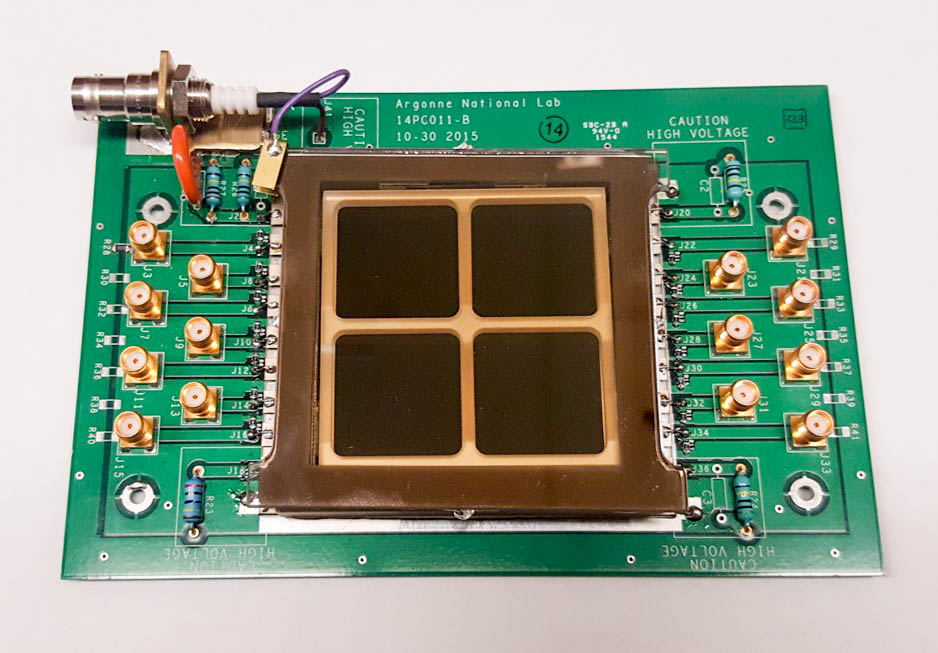
\includegraphics[scale=0.23]{fig/MCPs_assembly.png}
\caption{Completed 6$\times$6~cm$^2$ MCP-based photodetector attached to a 
circuit board, providing firm electrical connections.} \label{fig:MCP_assm}
\end{figure}

The microchannel plates used in the 6$\times$6~cm$^2$ MCP photodetector are 
diced from the next-generation large area (20$\times$20~cm$^2$) MCPs 
\cite{LAPPD,Craven-MCPs}, the world's largest commercially available MCPs.  
These next-generation MCPs are produced through a glass drawing process and 
functionalized through the ALD process. This is completely different from the 
production of traditional leaded glass MCPs. The glass drawing process uses 
borosilicate glass as the tube material, which is considerably less expensive 
than leaded glass and eliminates the chemical etching process required in the 
traditional method. This makes it much more cost-effective for MCP production.  
Here, we use standard borosilicate glass MCPs with 20~$\mu$m pore size, 60:1 
L/d (pore length to diameter) ratio and 8$^{\circ}$ bias angle relative to the 
MCP surface normal. The two MCPs are placed as the chevron configuration in the 
vacuum package, which reversed the bias angle to -8$^{\circ}$. 


\section{Rate capability measurement} \label{sec_proton_measurements}
The rate capability of MCP-based photodetectors is one of the most critical 
parameters for applications in high luminosity environments, such as the EIC.  
Due to the high resistive layer coating on ALD functionalized MCPs, the current 
in the MCP pores may not flow off fast enough when the MCP-based detector is 
exposed to high particle rates. This effect may cause severe charge saturation 
reducing the gain of the MCP-based photodetector, and limiting the detector 
performance. 
 
We investigated the rate capability of the 6$\times$6~cm$^2$ MCP-based 
photodetectors with the 120~GeV/c primary proton beam at Fermilab Test Beam 
Facility (FTBF). The beam is delivered as a slow spill with a 4~s duration once 
per minute with a maximum intensity of $~$10$^5$ particles per spill. The beam 
shape is circular with a diameter of 6~mm and a Gaussian density profile.  The 
beam intensity was close to a constant during each spill period. The incident 
proton beam was monitored by an upstream multiwire proportional counter to see 
the beam profile. Three plastic scintillators were used in coincidence as a 
trigger and to count the number of incident protons. A light-tight dark box was 
designed to hold the MCP-based photodetector in the beam path with the detector 
surface facing the beam direction. High voltage was applied to the MCPs through 
an external resistor voltage divider, and signals from the strip lines were 
read out through a DT5742 desktop digitizer \cite{Digitizer} produced by CAEN 
(Costruzioni Apparecchiature Elettroniche Nucleari S.p.A.) with a sampling rate 
of 5~GS/s. The digitizer is based on a switched capacitor array of DRS4 (Domino 
Ring Sampler) chips \cite{DRS}, 16 analog input channels, and one additional 
analog input for fast trigger.

During our experiment, the 120~GeV/c proton beam intensity was tuned to vary 
from 500 to 40,000 particles per spill. The beam rate was calculated using the 
number of triggers per spill and was corrected for the size of the beam spot by 
reconstructing the beam profile. The calculated beam rate varied from 3 to 
150~kHz/cm$^2$ corresponding to the monitored beam particle intensity. Figure 
\ref{fig:MCPs_gain_proton_beam} shows the gain of the MCP-based photodetector 
measured as a function of the beam rate. The measured gain of the investigated 
detector is stable up to a beam flux of 75~kHz/cm$^2$, and is still over 10$^7$ 
when the beam flux reaches 150~kHz/cm$^2$. Such a high rate capability of the 
MCP-based photodetector will be sufficient for EIC PID detectors at the 
proposed beam energies.
%, which are expected to work at a rate environment of  xxx Hz/cm$^2$.

\begin{figure}[tbp]
\centering 
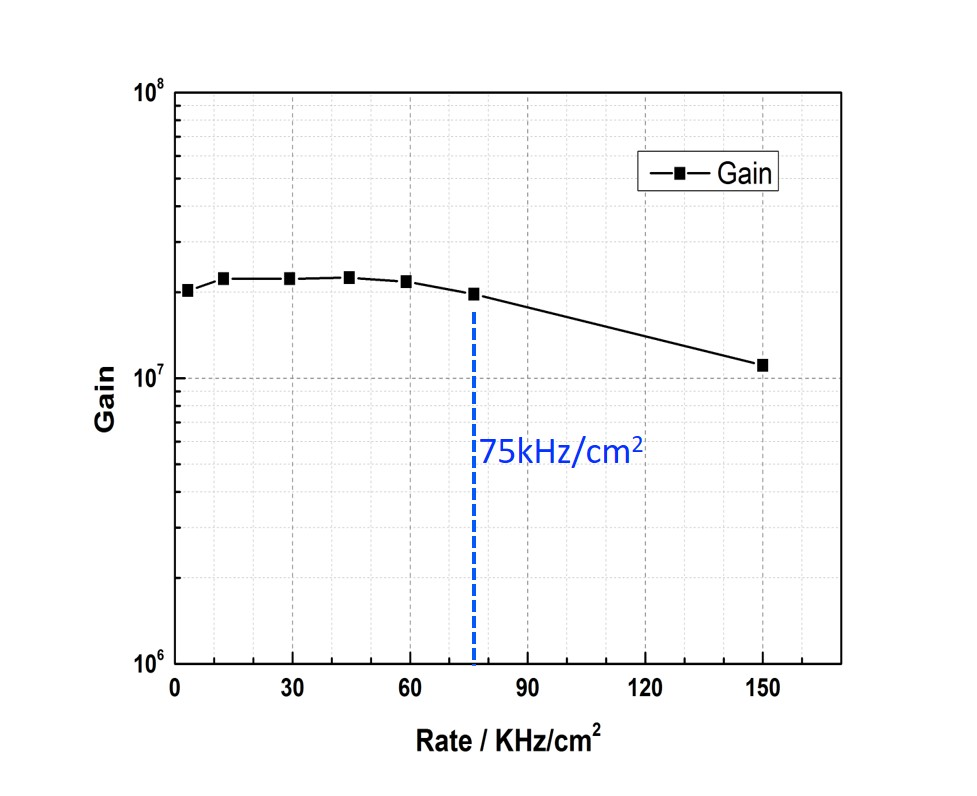
\includegraphics[scale=0.25]{fig/MCPs_gain_proton_beam.png}
\caption{Gain of the MCP-based photodetector as a function of the 120 GeV/c 
proton beam flux. The gain of the detector is stable up to beam flux of 75 
kHz/cm$^2$, and the gain is still over 10$^7$ at 150 kHz/cm$^2$. } 
\label{fig:MCPs_gain_proton_beam}
\end{figure}

\section{Magnetic field tolerance measurement}\label{sec_B_measurement}
In the EIC detector concepts, solenoid magnets with field strengths of 
1.5~Tesla are proposed. The imaging \u Cerenkov detectors (RICH, DIRC) and 
time-of-flight systems are designed to cover the area of the barrel and end 
caps for charged particle ($e$/$\pi$/$K$/$p$) separations. This compact design 
requires the photosensors to work properly in harsh environments with magnetic 
field strengths up to 1.5 Tesla. 

At ANL, a decommissioned superconducting magnet from a magnetic resonance 
imaging (MRI) scanner was acquired to test instruments for the muon g-2 
experiment \cite{Magnet}. The magnet provides a large bore with a diameter of 
68~cm and a very homogeneous field (7~ppb/cm), with a tunable strength of the 
magnetic field up to 4~Tesla. We have built a characterization system 
compatible with the solenoid magnet to test the performance of the 
6$\times$6~cm$^2$ MCP-based photodetector in a strong magnetic field 
environment. The MCP photodetector was fixed in a custom built non-magnetic, 
light-tight dark box. The dark box was held on a test platform with the 
detector surface normal to the direction of magnetic field. The position of the 
dark box was adjusted so that the center of the MCP photodetector was 
well-aligned with the center of the solenoid magnet. A rotation mechanism was 
also integrated with the system, allowing rotation of the MCP-based 
photodetector with an angle $\theta$, as shown in Figure 
\ref{fig:MCPs_theta_rotation}. A 405 nm light-emitting diode (LED) was used as 
the light source and was introduced to the surface of the MCP photodetector 
through an optical fiber.  High voltage was applied to the MCPs from a supply 
with variable voltage control, and signals from the strip lines were read out 
through the CAEN DT5742 desktop digitizer.

\begin{figure}[tbp]
\centering 
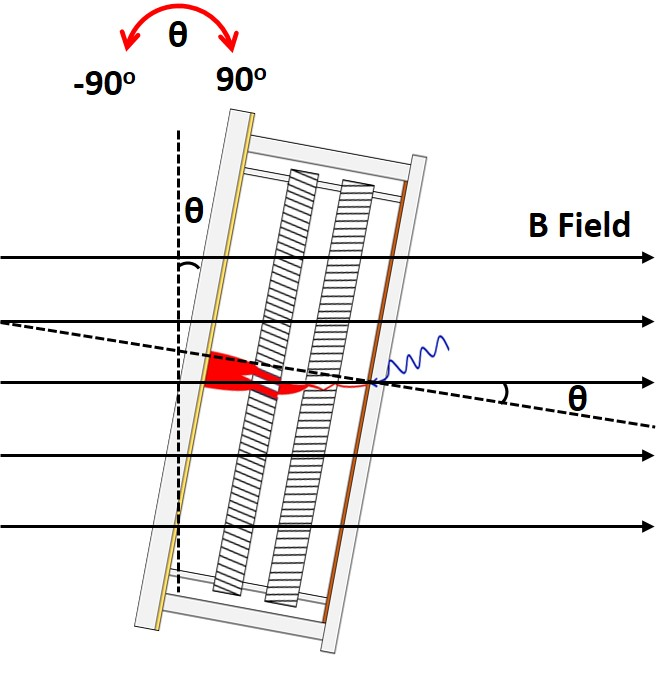
\includegraphics[scale=0.27]{fig/MCPs_theta_rotation.png}
\caption{Schematic of the rotation mechanism of the MCP-based photodetector 
with angle $\theta$ relative to the magnetic field direction during the 
measurement.} \label{fig:MCPs_theta_rotation}
\end{figure}

\subsection{Magnetic field strength dependence}\label{subsec_HV}
\begin{figure}[tbp]
\hspace{-1.0 cm} 
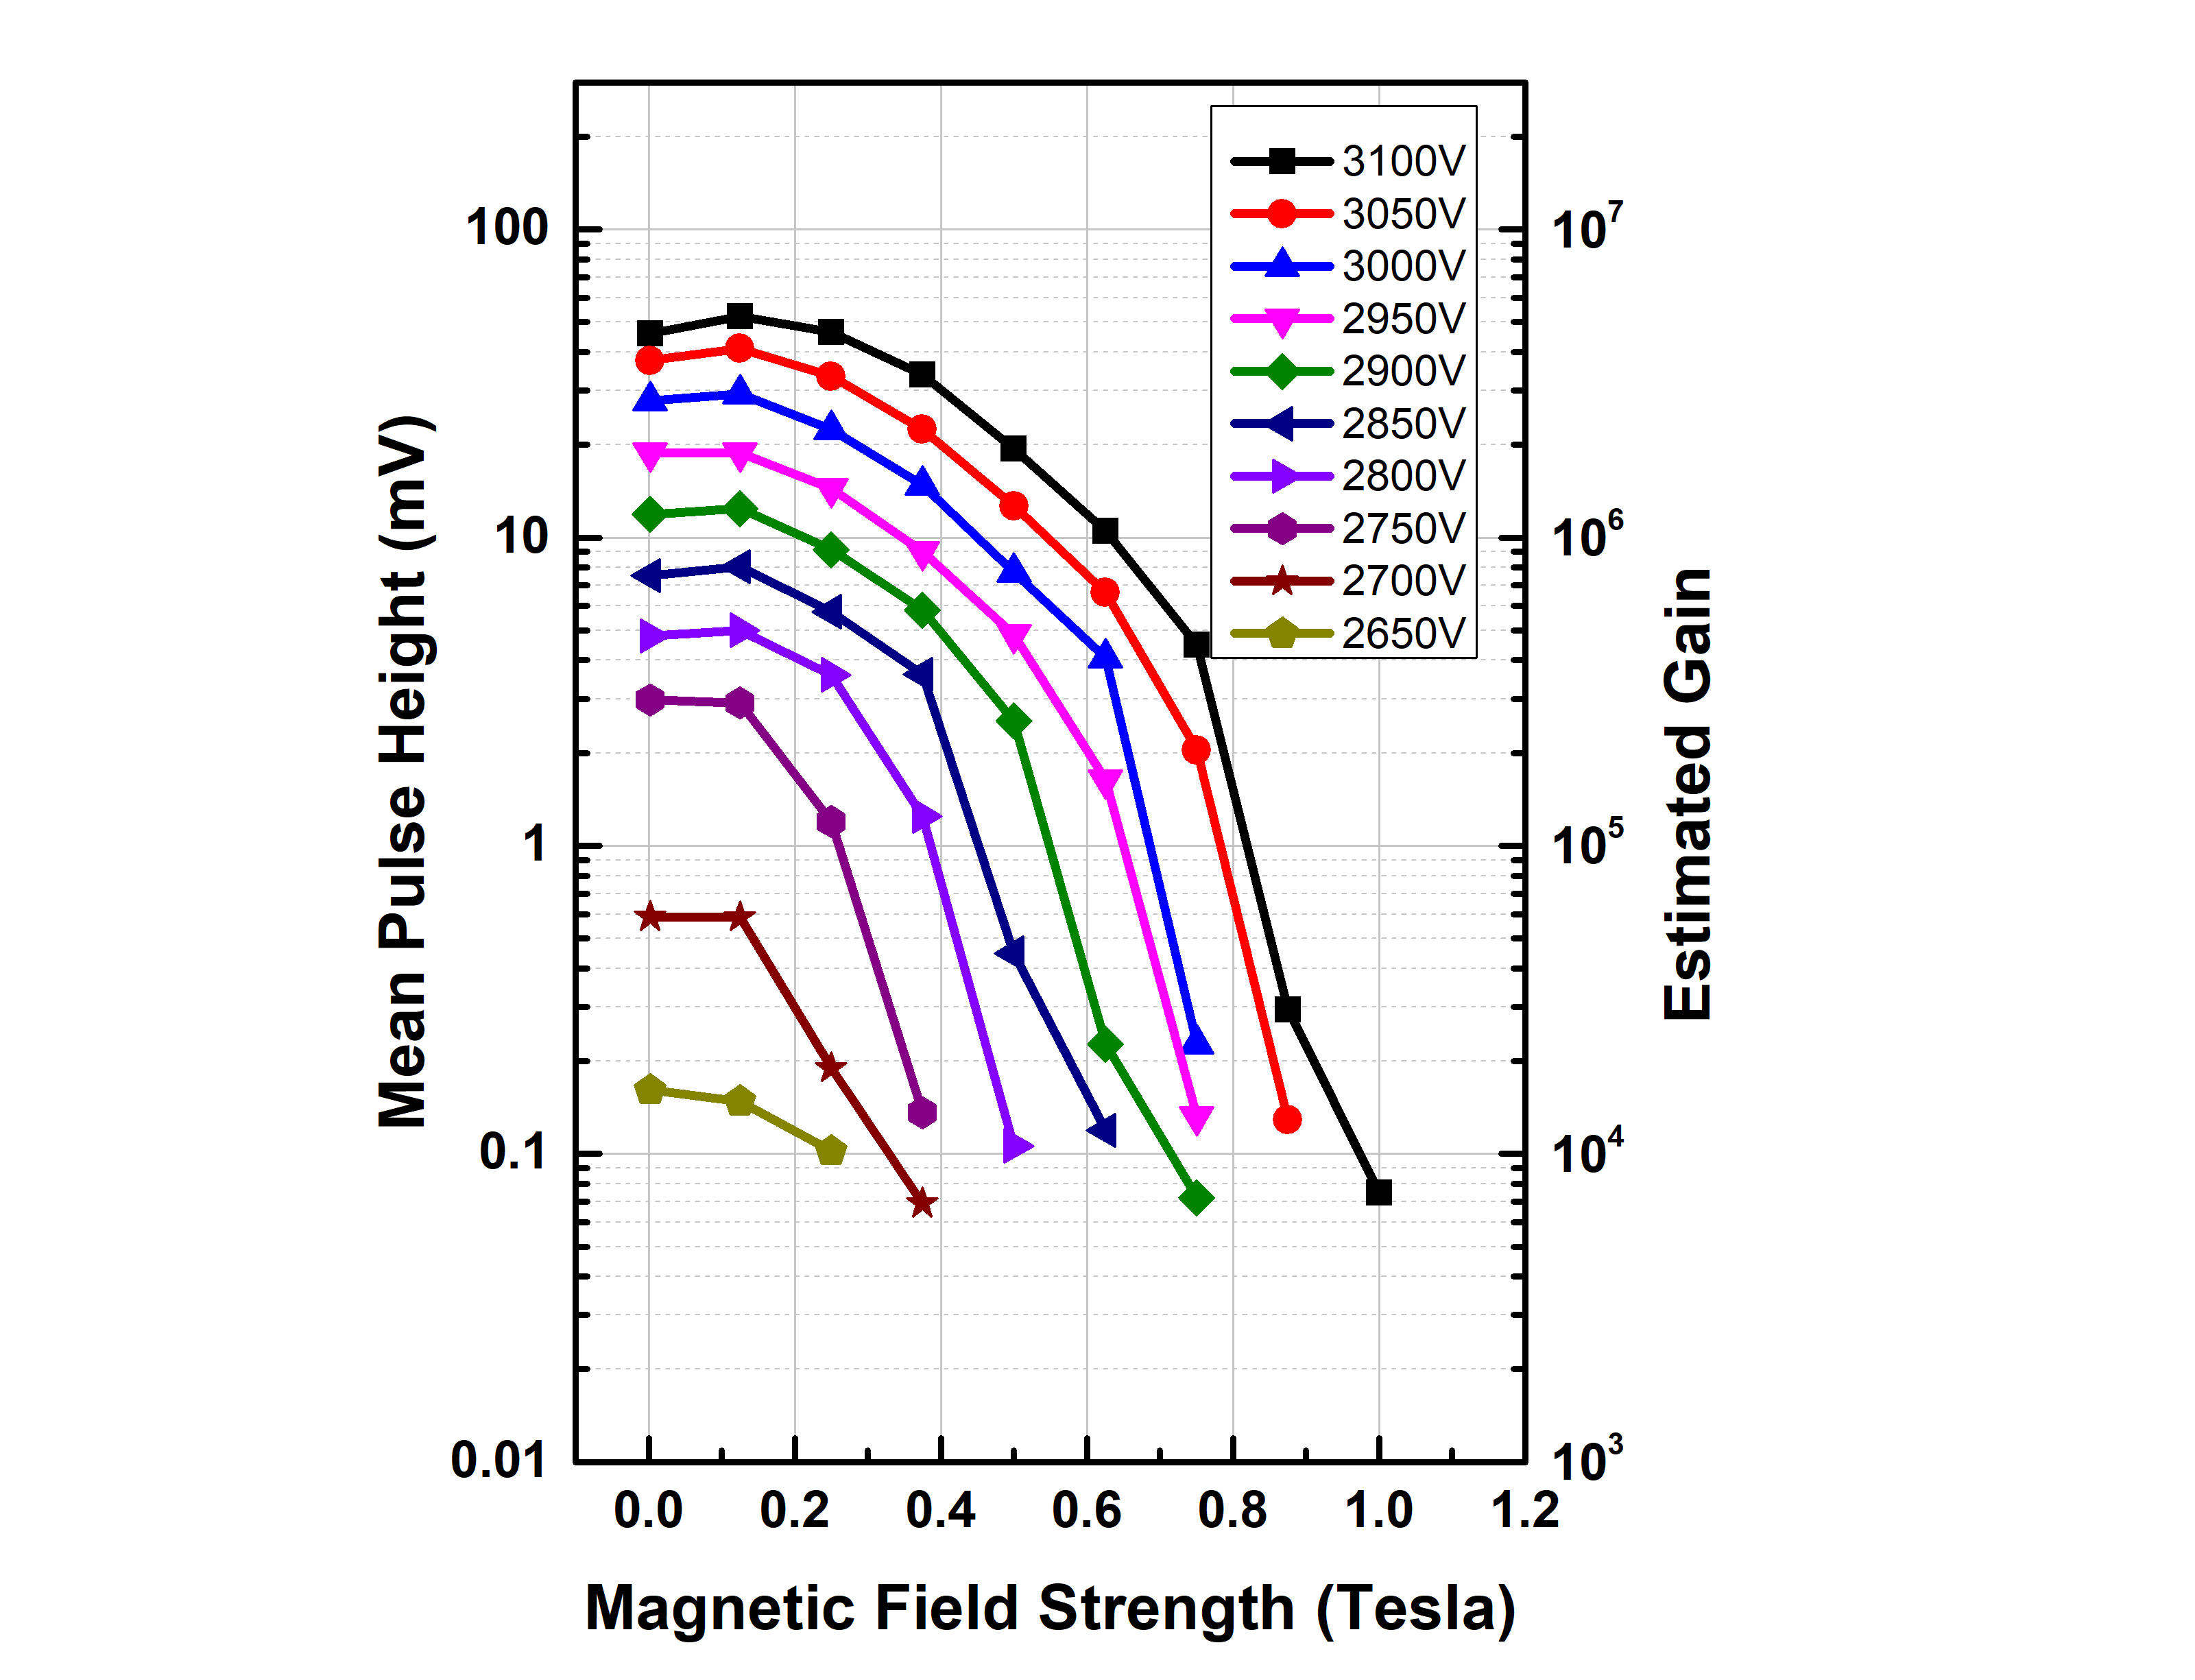
\includegraphics[scale=0.1]{fig/MCPs_gain_B_HV.png}
\caption{Dependence of the MCP-based photodetector gain on the magnetic field 
strength at different high voltages.} \label{fig:MCPs_gain_B_HV}
\end{figure}

The dependence of the MCP photodetector performance on the magnetic field 
strength was done at a rotation angle $\theta$ = 0$^{\circ}$, i.e., where the 
direction of the magnetic field is normal to the surface of the MCP-based 
photodetector. We measured the gain of the investigated MCP photodetector in 
various magnetic field strengths with different bias voltages. The results are 
presented in Figure \ref{fig:MCPs_gain_B_HV}. The gain is calculated based on 
integrated charge in a pulse normalized to a single photoelectron. At a fixed 
bias high voltage, the gain of the MCP photodetector increases slightly as the 
magnetic field strength increases to 0.2~T, decreases as the magnetic field 
strength continues to increase, and eventually breaks down at a fixed magnetic 
field strength of $\sim$~0.8~T. In the same magnetic field environment, the 
gain of the MCP photodetector increases as the high voltage increases. This 
behavior is similar to our previous measurement of the MCP photodetectors 
without applying a magnetic field. 


\subsection{Magnetic field angle dependence}\label{subsec_theta}

\begin{figure}[tbp]
\centering 
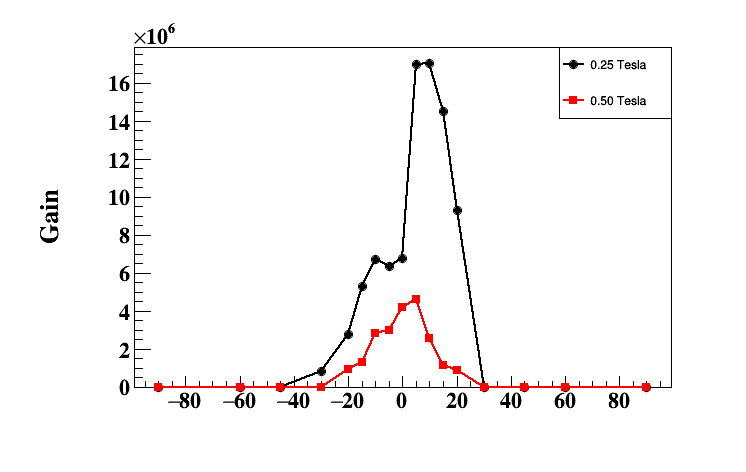
\includegraphics[scale=0.35]{fig/MCPs_gain_theta_B.png}
\caption{Gain of the MCP photodetector as a function of the rotation angle 
   $theta$ relative to the direction of magnetic field. The two peaks around 
-8$^{\circ}$ and 8$^{\circ}$ indicates the effect due to the 8$^{\circ}$ bias 
angle of the MCPs. Note that the intensities of these two peaks are not the 
same due to the different effect from top and bottom MCPs.} 
\label{fig:MCPs_gain_theta_B}
\end{figure}
The angular dependence of the MCP photodetector was additionally studied by 
rotating the MCP photodetector along with angle $\theta$ relative to the 
magnetic field direction, as shown in Figure \ref{fig:MCPs_gain_B_HV}. We fixed 
the biased high voltage at 3000 V on the photodetector and rotated the 
photodetector from -90$^{\circ}$ to 90$^{\circ}$ for a full range of angle 
measurements. Figure \ref{fig:MCPs_gain_theta_B} presents the gain of the MCP 
photodetector measured as a function of the rotation angle $\theta$ at two 
magnetic field strengths of 0.25 and 0.5~Tesla. The MCP photodetector almost 
does not provide detectable signals when $\theta$~$\leq$~-30$^{\circ}$ or 
$\theta$~$\geq$~30$^{\circ}$.  Within 
-30$^{\circ}$~$\leq$~$\theta$~$\leq$~30$^{\circ}$, there are two gain peaks at 
$\theta$ = $\pm$8$^{\circ}$, which are due to the chevron configuration of two 
MCPs inside the photodetector. The gain reaches a maximum when the pore of 
either MCP is well-aligned with the magnetic field direction. The intensities 
of the two peaks are different, which is due to the different effect from the 
top and bottom MCPs.



\subsection{Design optimization of MCP-based photodetector}\label{subsec_opt}
In the EIC experiment, a 1.5~Tesla solenoid magnet will be used for tracking 
charged particles. The magnetic field tolerance requirement varies from 
detector to detector depending on their distances from the interaction point 
and the magnetic field direction. From our measurement, the 6$\times$6~cm$^2$ 
MCP-based photodetector has shown a good magnetic field tolerance of up to 0.8 
Tesla, comparable to that of current commercially available MCP-PMTs 
($\sim$~1.0~T) with similar pore size \cite{MCPs-B}. Here, we must emphasize 
that the current LAPPD design is not yet optimized for magnetic field tolerant 
applications. The distances between the photocathode, MCPs, and the anode are 
relatively large in the LAPPD design. For instance, the spacings between the 
photocathode and the top MCP of 2~mm and spacings between the bottom MCP and 
the anode of 3.2~mm \cite{Wang-MCPs}. To optimize for a magnetic field 
environment, these distances should be reduced to minimize the electron transit 
distance. Meanwhile, MCP photodetectors with smaller pore sizes have shown 
better magnetic field tolerance than those with larger pore sizes
\cite{MCPs-B, Lehmann, Ilieva}. A redesign of the current LAPPD configuration 
with smaller pore sizes (e.g.  10~$\mu$m or even 5~$\mu$m) and reduced 
distances between the PMT elements would improve its magnetic field tolerance. 

\section{Conclusions}
We have described the current design of 6$\times$6~cm$^2$ microchannel plate 
photodetectors with the next-generation MCPs functionalized through atomic 
layer deposition process. The rate capability and magnetic field tolerance of 
these photodetectors were tested at Fermilab's 120 GeV proton beam and 
Argonne's 4~Tesla magnetic field facility. The photodetectors exhibit stable 
performance for rates up to 75~kHz/cm$^2$ and magnetic field tolerance for 
fields up to 0.8~Tesla. The magnetic field angle dependence was also measured, 
showing enhanced performance at $\pm$8$^{\circ}$ tilt angle due to the original 
MCP 8$^{\circ}$ bias angle. The magnetic field tolerance of these detectors 
could be further improved by using smaller pore size MCPs and redesigning the 
package with reduced distances between the photocathode, MCPs, and anode.
 

\input acknowledgment.tex  

\begin{thebibliography}{99}

\bibitem{EIC}
A. Accardi et al., Electron Ion Collider: The Next QCD Frontier, Eur. Phys. J.  
A 52 (2016) 268.

\bibitem{LRP}
A. Aprahamian et al., Reaching for the horizon: The 2015 long range plan for 
nuclear science, 2015. 

\bibitem{RICH}
C.P. Wong et al., Modular focusing ring imaging Cherenkov detector for 
electron-ion collider experiments, Nucl. Instr. and Meth. A 871 (2017) 13.

\bibitem{RICH2}
A. Del Dotto et al., Design and R{\&}D of RICH detectors for EIC experiments, 
   Nucl. Instr. and Meth. A (2017).

\bibitem{DRIC}
G. Kalicy et al., High-performance DIRC detector for the future Electron Ion 
Collider experiment, JINST 11 (2016) C07015.

\bibitem{LAPPD}
   M. Minot et al., Pilot production {\&} commercialization of LAPPD$^{TM}$, 
   Nucl.  Instr.  and Meth. A 787 (2015) 78.

\bibitem{LAPPD2}
B. Adams et al., A brief technical history of the Large-Area Picosecond 
Photodetector (LAPPD) Collaboration, 2016 arXiv:1603.01843.

\bibitem{LAPPD-ANL}
J. Xie et al., Development of a small form-factor (6cm$\times$6 cm) picosecond 
photodetector as a path towards the commercialization of large area devices, 
in: Proceeding of ``The Technology and Instrumentation in Particle Physics 
2014", PoS 2014.

\bibitem{ANL-MCPs}
J. Xie et al., Design and fabrication of prototype 6$\times$6 cm$^2$ 
microchannel plate photodetector with bialkali photocathode for fast timing 
applications, Nucl. Instr. and Meth. A 784 (2015) 242.

\bibitem{Wang-MCPs}
J. Wang et al., Development and testing of cost-effective, 6cm$\times$6cm 
MCP-based photodetectors for fast timing applications, Nucl. Instr. and Meth.  
A 804 (2015) 84.

\bibitem{Wang-MCPs2}
J. Wang et al., Design improvement and bias voltage optimization of glass-body 
microchannel plate picosecond photodetector, IEEE Trans. Nucl. Sci. 64 (2017) 
1871.

\bibitem{Craven-MCPs}
C. Craven et al., Recent advances in Large Area Micro-Channel Plates and 
LAPPD$^{TM}$, Springer Proceedings in Physics (2017).

\bibitem{Xia-MCPs}
L. Xia et al., Systems and methods for forming microchannel plate (MCP) 
photodetector assemblies, U.S. Patent 9704900 B1, July 11, 2017.

\bibitem{Digitizer}
DT5742 desktop digitizer 
\url{http://www.caen.it/jsp/Template2/CaenProd.jsp?parent=14&idmod=651}

\bibitem{DRS}
   DRS chip developed at Paul Scherrer Institut, Switzerland \url{
https://www.psi.ch/drs}

\bibitem{Magnet}
4 Tesla Magnet Facility 
\url{https://www.anl.gov/hep/group/4-tesla-magnet-facility}

\bibitem{MCPs-B}
A. Lehmann et al., Performance studies of microchannel plate PMTs in high 
magnetic fields, Nucl. Instr. and Meth. A 595 (2008) 173.

\bibitem{Lehmann}
A. Lehmann et al., Systematic studies of micro-channel plate PMTs, Nucl.  
Instr. and Meth. A 639 (2011) 144.

\bibitem{Ilieva}
Y. Ilieva et al., MCP-PMT studies at the High-B test facility at Jefferson Lab, 
JINST 11 (2016) C03061.

\end{thebibliography}

\end{document}

